\documentclass{article}

% Language setting
% Replace `english' with e.g. `spanish' to change the document language
\usepackage[english]{babel}

% Set page size and margins
% Replace `letterpaper' with`a4paper' for UK/EU standard size
\usepackage[letterpaper,top=2cm,bottom=2cm,left=3cm,right=3cm,marginparwidth=1.75cm]{geometry}

% Useful packages
\usepackage{amsmath}
\usepackage{graphicx}
\usepackage[colorlinks=true, allcolors=blue]{hyperref}

\title{Esercizio NuSMV Produttori e Consumatori}
\author{Ruben Castelluccio}

\begin{document}
\maketitle


\section{Introduzione}
L'esercizio consiste nell'Analisi mediante NuSMV per il problema Produttore - Consumatore.
\\ Si richiede di analizzare 3 diversi modelli di Produttore e Consumatore dove il Buffer è sempre definito a N posizioni:
\begin{itemize}
    \item Primo Setting: 1 Produttore, 1 Consumatore, Buffer a N posizioni;
    \item Secondo Setting: 1 Produttore, 2 Consumatori, Buffer a N posizioni;
    \item Terzo Setting: P Produttori, C Consumatori, Buffer a N posizioni.
    \end{itemize}
    Si richiede per ciascun Setting il Modelling Convenience, valutazione della difficoltà per l'implementazione utilizzando la simulazione interattiva di NuSMV.
    \\Si definisce il buffer come un contatore indicato dalla variabile \textit{bufsize} su cui si possono fare al più 3 inserimenti consecutivi da parte del produttore, inoltre i processi devono procedere, non posso fermarsi in uno stato, a meno che le condizioni relative al buffer non lo consentino. 
    \\Inoltre viene definita una sezione per ogni setting denominata \textit{Analisi Generale} in cui vengono riportati i risultati in seguito all'esecuzione dei seguenti comandi:
    \begin{itemize}
        \item \textit{check\_fsm}: verifica assenza di deadlock pertanto per ongi stato esiste un successore;
        \item \textit{print\_reachable\_states -v}: costruzione stati raggiungibili.
    \end{itemize}
\clearpage
\section{Setting 1}
Nell'implementazione per il Setting 1 si definiscono un processo \textit{prod}, un processo \textit{cons} e una variabile globale condivisa dai 2 processi \textit{bufsize}.
\\ Il processo produttore è inizializzato in uno stato in cui pensa \textit{think}, successivamente produce e infine inserisce nel buffer mediante \textit{put} se \textit{bufsize} è inferiore a 3, altrimenti si metterà in attesa che il processo consumatore consumi.
\\ Il processo consumatore è inizializzato in uno stato di attesa \textit{wait} e verifica che il produttore abbia almeno eseguito un inserimento nel buffer per poter consumare e se tale condizione è soddisfatta andrà nello stato di \textit{get}, altrimenti rimane in attesa. Successivamente andrà nello stato in cui pensa \textit{think} per poi rimettersi in attesa. 
\begin{figure}[h] 
\centering
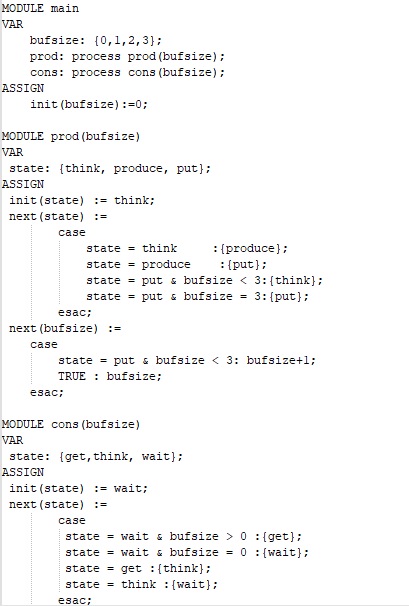
\includegraphics[scale=0.8]{setting11.png}
\end{figure}
\begin{figure}[h] 
\centering
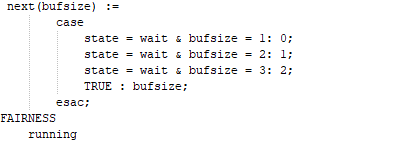
\includegraphics[scale=0.9]{setting12.png}
\end{figure}
\subsection{Analisi Generale}
    \begin{itemize}
        \item \textit{check\_fsm}: l'assenza di deadlock è rispettata;
        \item \textit{print\_reachable\_states -v}: il numero di stati raggiungibili è pari a 36, analogamente a quanto riscontrato dal Reachability Graph per le reti PT per il Setting 1 mediante GreatSPN.
    \end{itemize}
\subsection{Modelling Convenience}
La principale difficoltà nell'implementazione del Setting 1 ha riguardato la definizione del buffer come un contatore limitato con un upper bound di 3 posizioni.
\clearpage
\section{Setting 2}
Nell'implementazione del Setting 2 sono definiti un processo \textit{prod} e 2 processi \textit{cons} e una variabile condivisa \textit{bufsize}. In maniera del tutto analoga al Setting 1 sono definiti i processi ad eccezzione di definire un ulteriore consumatore \textit{cons2}.
\begin{figure}[h] 
\centering
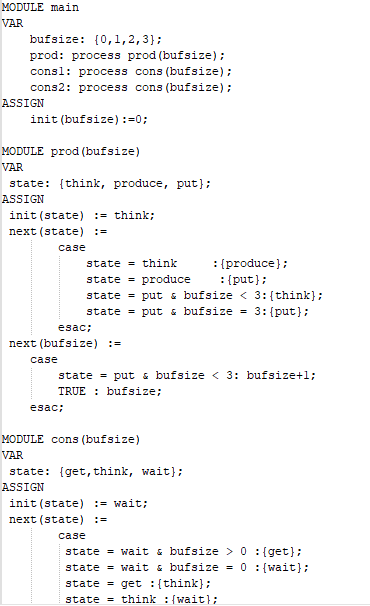
\includegraphics[scale=0.8]{setting21.png}
\end{figure}
\begin{figure}[h] 
\centering
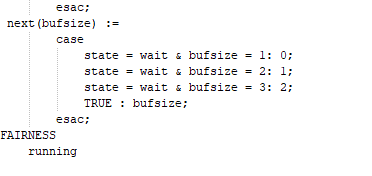
\includegraphics[scale=0.9]{setting22.png}
\end{figure}
\subsection{Analisi Generale}
    \begin{itemize}
        \item \textit{check\_fsm}: l'assenza di deadlock è rispettata;
        \item \textit{print\_reachable\_states -v}: il numero di stati raggiungibili è pari a 108, analogamente a quanto riscontrato dalla Reachability Graph per le reti PT per il Setting 2 - Scalatura per Replicazione mediante GreatSPN.
    \end{itemize}
\clearpage
\section{Setting 3}
Nell'implementazione del Setting 3 sono definiti 2 processi \textit{prod} e 2 processi \textit{cons} e una variabile condivisa \textit{bufsize}.
\begin{figure}[h] 
\centering
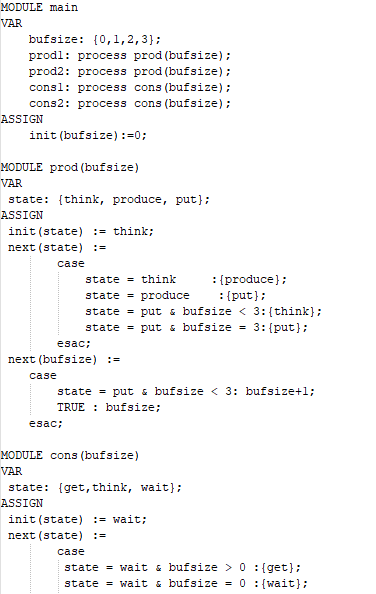
\includegraphics[scale=0.8]{setting31.png}
\end{figure}
\begin{figure}[h] 
\centering
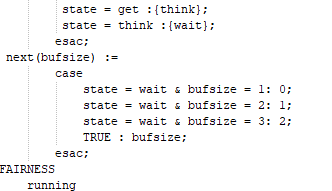
\includegraphics[scale=0.9]{setting32.png}
\end{figure}
\subsection{Analisi Generale}
    \begin{itemize}
        \item \textit{check\_fsm}: l'assenza di deadlock è rispettata;
        \item \textit{print\_reachable\_states -v}: il numero di stati raggiungibili è pari a 324, analogamente a quanto riscontrato dalla Reachability Graph per le reti PT per il Setting 3 - Scalatura per Replicazione mediante GreatSPN.
    \end{itemize}
\subsection{Modelling Convenience}
La principale difficoltà nell'implementazione del Setting 3 ha riguardato la definizione di P produttori e C consumatori rispettivamente a 2 processi produttori e 2 processi consumatori dato che non è possibile parametrizzare il numero di processi.
\end{document}